%   Filename    : chapter_4.tex 
\ensuremath{\pm}


\chapter{Preliminary Results/System Prototype}
This chapter presents the preliminary results between the comparison of trained machine learning models: Logistic Regression, Random Forest,  Decision Trees, Support Vector Machine (SVM), and k-nearest Neighbors (KNN).  This chapter will also present the model evaluation and the comparison of model performance. 

\section{Data Summary}
\subsection{Dataset Overview}

The dataset contains the morphological measurements collected from the 77 male and 72 female T. granosa samples. The morphological characteristics included in the dataset are the length, width, height, rib count, hinge length, and distance between the umbos. Additional ratio-based characteristics, such as Length-to-Width ratio, and Length-to-Height ratio, were computed to take into consideration the size variations. These ratios were calculated by dividing the shell length by the shell width and height, respectively. 

\begin{figure}[!htbp]
	\centering
	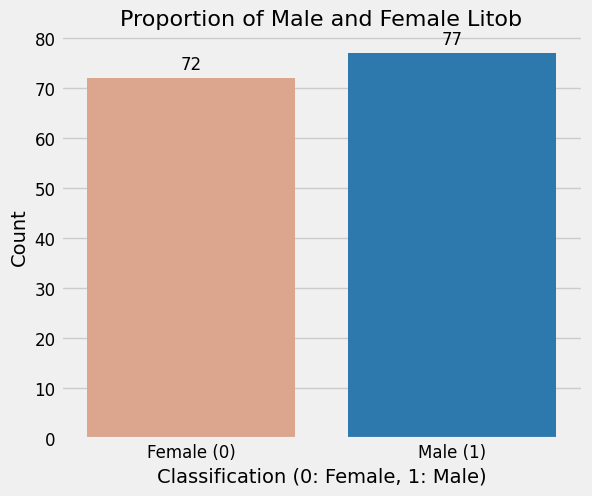
\includegraphics[width=0.6\textwidth]{figures/test-train.png}
	\caption{Proportion of Male and Female Data}
	\label{fig:test-train}
\end{figure}

\subsection{Preprocessing Results}

\begin{table}[H]
	\centering
	\resizebox{\linewidth}{!}{ 
		\begin{tabular}{lccc}
			\hline
			\textbf{Feature} & \textbf{$Mean \pm SD$} & \textbf{Min} & \textbf{Max}  \\ \hline
			Length              & $46.41 \pm 5.01$ & 38.050000 & 64.800000  \\
			Width               & $35.66 \pm 3.78$ & 28.250000 & 45.500000  \\
			Height              & $32.10 \pm 3.59$ & 23.350000 & 45.050000 \\
			Rib count           & $19.65 \pm 0.88$ & 17.000000 & 22.000000  \\
			Length (Hinge Line) & $28.06 \pm 4.24$ & 20.050000 & 43.050000  \\
			Distance Umbos      & $3.25 \pm 2.85$ & 1.050000 & 35.050000  \\
			LW\_ratio            & $1.30 \pm 0.07$ & 1.114710 & 1.692185  \\
			LH\_ratio            & $1.45 \pm 0.10$ & 1.191919 & 1.844398  \\
			 \hline
		\end{tabular}
	}
	\caption{ Descriptive statistics of the T. granosa features}
	\label{tab:descriptive-stat}
\end{table}

The preprocessing of the data includes data cleaning, feature engineering, and encoding. Any missing data entries were removed throughout the data cleaning process. The LW and LH ratios were calculated and added by feature engineering to standardize size variations among the samples while maintaining significant morphological patterns. Additionally, a categorical label was encoded using binary values. It was done by indicating male as 1 and female as 0. As for the final preparation, the dataset was split into 70\% as the training and 30\% as testing to ensure balanced male and female sample representation in the training set as well as in testing sets.

\section{Comparison of Model Performance}
\begin{figure}[!htbp]
	\centering
	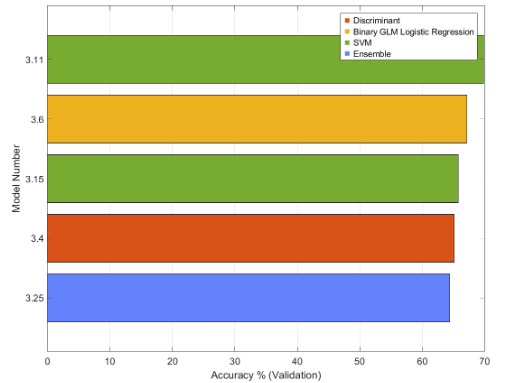
\includegraphics[width=0.6\textwidth]{figures/compare-models.png}
	\caption{Comparison of Model Performance}
	\label{fig:compare-models}
\end{figure}

\subsection{Performance Evaluation}

To evaluate the performance of the different models used, the effectiveness of the models were evaluated and compared in predicting the sex of the T.granosa based on morphological traits. The use of performance metrics such as accuracy, precision, recall, and F1-score is used to evaluate the performance of the different models. By analyzing the performance metrics the researchers can identify the most effective and best model for the classification of male and female T.granosa. 


\begin{table}[H]
	\centering
	\resizebox{\linewidth}{!}{ 
		\begin{tabular}{lccccc}
			\hline
			\textbf{Model} & \textbf{Accuracy (Validation)} & \textbf{ Weighted Precision} & \textbf{ Weighted Recall} & \textbf{Weighted F1-score} & \textbf{Training Time (sec)} \\ \hline
			Linear SVM          & 69.80(\%) & 69.82(\%) & 69.80(\%) & 69.73(\%) & 2.354 \\
			Binary GLM Logistic Regression    & 67.11 (\%) & 67.16(\%) & 67.11(\%) & 66.99(\%) & 1.9415 \\
			Medium Gaussian SVM       & 65.77(\%) & 65.77(\%) & 65.77(\%) & 65.69 (\%) & 1.0323 \\
			Linear Discriminant       & 65.10(\%) & 65.22(\%) & 65.10(\%) & 64.86(\%) & 2.333\\
			Subspace Discriminant     & 64.43(\%) & 64.50(\%) & 64.43(\%) & 64.23(\%) & 7.708 \\ \hline
		\end{tabular}
	}
	\caption{Model Performance Comparison}
	\label{tab:model-performance}
\end{table}

Table~\ref{tab:model-performance} presents the comparison results of machine learning models on the morphological traits of the combined  male and female T.granosa datasets. The results indicate that all models demonstrated moderate to high performance in predicting male and female, with accuracies ranging between 64.43\% to 69.80\%. 


\subsection{Confusion Matrix Analysis}
\begin{figure}[!htbp]
	\centering
	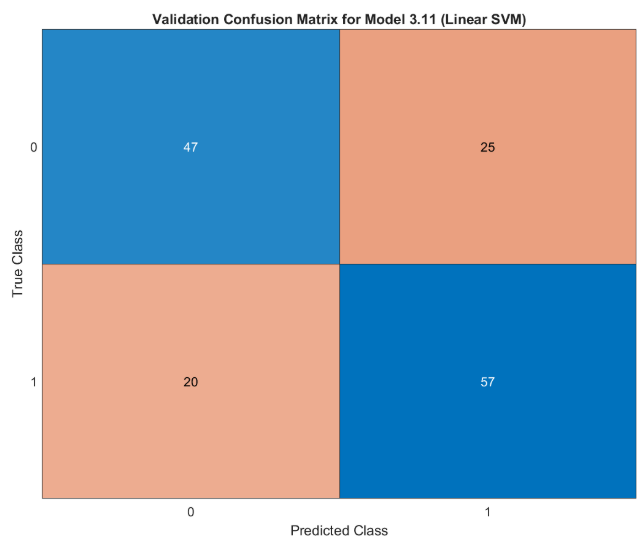
\includegraphics[width=0.6\textwidth]{figures/confusion-matrix.png}
	\caption{Confusion Matrix of Linear SVM}
	\label{fig:confusion-matrix}
\end{figure}

Figure ~\ref{fig:confusion-matrix} shows the confusion matrices that allow for a detailed breakdown of classifier predictions including true positives (correctly identified females), true negatives (correctly identified males), false positives (males incorrectly classified as females), and false negatives (females incorrectly classified as males).

Linear SVM being the best performing model had achieved 57 true positives and 47 true negatives. However, there were also 25 false positives and 20 false negatives. This indicates that the model did not accurately differentiate  between male and female, agreeing to its accuracy with (69.80\%). The large number of wrongly classified data points can only indicate that while Linear SVM is the best model compared to others it still suffers from the complexity of this dataset. 


\subsection{Feature Importance Analysis}



